\section{Introdução}

Este trabalho aborda o desenvolvimento de um controle supervisório para uma planta industrial com processo de  manufatura. A figura \ref{fig:processo} apresenta uma visão da planta industrial a ser modelada e simulada.

%\subsection{Processo industrial de manufatura}

\begin{figure}[h]%
	\centering
	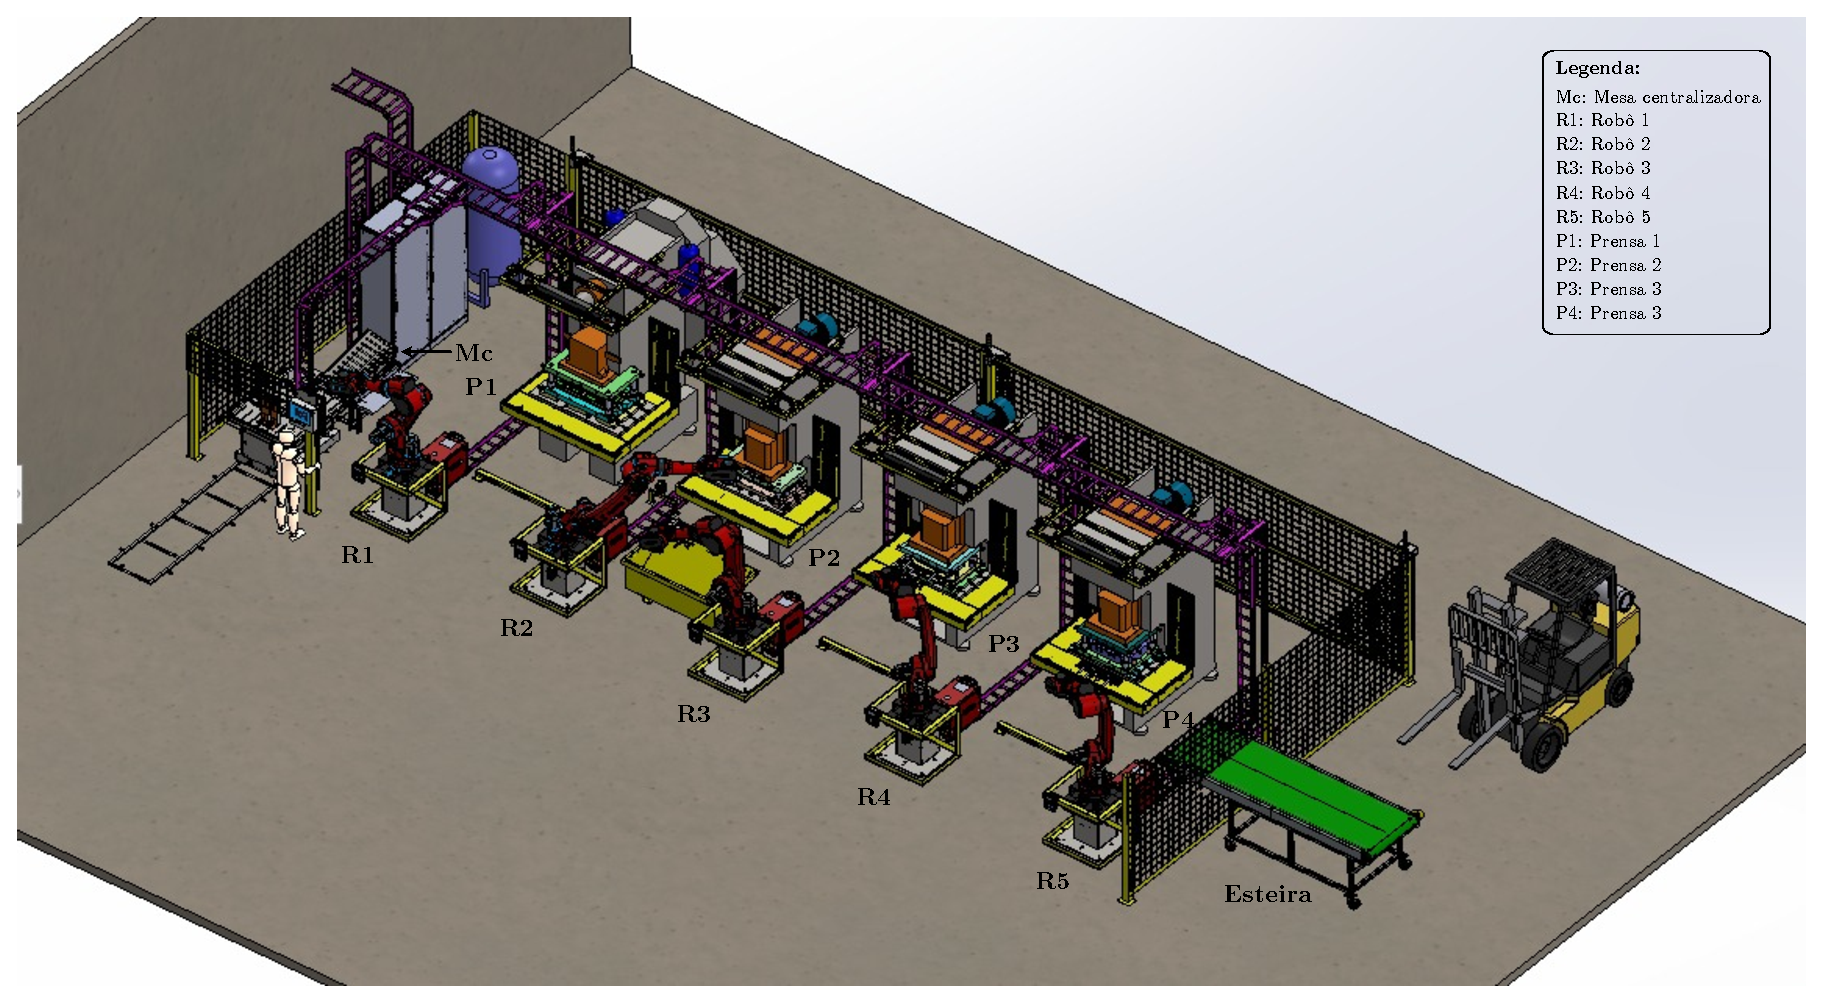
\includegraphics[width=0.75\textwidth]{imagens/processo.eps}
	\caption{Planta industrial}\label{fig:processo}
\end{figure}

A planta é composta por:
\begin{itemize}
    \item Mesa centralizadora com teste de chapa;
    \item 5 robôs manipuladores;
    \item 4 prensas;
    \item Esteira para destinação final das peças;
\end{itemize}

Partindo de uma posição segura para todos os robôs, o primeiro robô inicia sua movimentação para pegar a chapa da mesa centralizadora e levar até a primeira prensa, ao finalizar o processo o segundo robô faz o transporte até a segunda prensa e assim sucessivamente até o robô 4, que entrega a peça ao robô 5 e esse insere na ultima prensa e realiza a entrega o produto pronto para a esteira. 

O controle modular será aplicado dada a possibilidade de tratar individualmente cada etapa do conjunto descentralizando em subplantas e especificações locais, formando os supervisores locais. Se não conflitarem entre si, irão compor um supervisor completo com comportamento equivalente a um supervisor monolítico.